\documentclass[spanish]{book}
\usepackage{titlesec}

%Quitar páginas en blanco
\let\cleardoublepage\clearpage
\usepackage{etoolbox}
\makeatletter
\patchcmd{\@endpart}{\vfil\newpage}{\par}{}{}
\makeatother

%\usepackage[spanish]{babel} ¡Esto estaba interfiriendo con las flechitas de los \tikspicture

\renewcommand{\contentsname}{Índice}
\renewcommand{\partname}{Parte}

\titleformat{\chapter}[display]
{\normalfont\huge\bfseries}{}{0pt}{\Huge\thechapter.~}

\titleformat{name=\chapter,numberless}[display]
{\normalfont\huge\bfseries}{}{0pt}{\Huge}
\renewcommand{\chaptermark}[1]{\markboth{{} \thechapter: #1}{}}



\usepackage[bookmarks,bookmarksopen,bookmarksdepth=3]{hyperref}
\usepackage{graphicx}
\usepackage{wrapfig}
\usepackage{float}
\usepackage{subcaption}
\usepackage[left=4cm, right=4cm]{geometry}
\usepackage{enumitem}
\usepackage{palatino}
\usepackage{parskip}
\usepackage{array}%This is used in a table
\usepackage{amsthm}
\usepackage{amssymb}
\usepackage[nointegrals]{wasysym}%I was getting some problem "\iint already defined"
\usepackage{amsmath}
\usepackage{tikz}
\usepackage{tikz-cd}
\usetikzlibrary{%
	matrix,%
	calc,%
	arrows,%
	shapes,
	decorations.markings
}
\tikzstyle{line}=[draw]
%\usepackage[style=nature]{biblatex}
\usepackage[nottoc,numbib]{tocbibind}%This is to include the References in the ToC. For some reason it is not working so I add it manually at the end of the document.
%\addbibresource{bib.bib}

\hypersetup{%Remove red rectangles on hyperlinks
	colorlinks=false,
	hidelinks
}

\theoremstyle{definition}
\newenvironment{Proof}[1][Proof]%Proof within proof
{\proof[#1]\leftskip=1cm\rightskip=1cm}{\endproof}

\newtheorem*{defn}{Definición}
\newtheorem{defs}{Definiciones}
\newtheorem*{lema}{Lema}
\newtheorem*{obs}{Observación}
\newtheorem*{teo}{Teorema}
\newtheorem*{prop}{Proposición}
\newtheorem{coro}{Corolario}
\newtheorem*{coro*}{Corolario}
\newtheorem*{ejer}{Ejercicio}
\newtheorem*{ejem}{Ejemplo}
\newtheorem*{pregunta}{Pregunta}

\newcommand{\R}{\mathbb{R}}
\newcommand{\Z}{\mathbb{Z}}
\newcommand{\N}{\mathbb{N}}
\newcommand{\C}{\mathbb{C}}
\newcommand{\Q}{\mathbb{Q}}
\newcommand{\T}{\mathbb{T}}
\newcommand{\K}{\mathbb{K}}
\DeclareMathOperator{\coker}{coker}
\DeclareMathOperator{\img}{img}

\title{Notas de Topología Algebraica}
\author{Prof. Luis Jorge Sánchez Saldaña\\ \\ Notas por Dani}

\begin{document}
	\maketitle
	\tableofcontents
	
\part{Grupo fundamental}
	
\part{Espacios cubrientes}
	
\part{Homología}
\chapter{Álgebra Homológica}
\section{Conceptos básicos}
	En este capítulo $R$ denotará un anillo asociativo con unidad (no necesariamente conmutativo). Normalmente pensaremos que es alguno de los siguientes: $\Z, \Q, \R$.
	
	Recordemos que un $R$-módulo es básicamente un espacio vectorial pero los escalares están $R$.
	\begin{defn}
		Un \textbf{$R$-complejo de cadenas} es una sucesión de $R$-módulos y homomorfismos
		\[\begin{tikzcd}
			(C_\bullet,\partial):= \quad \cdots \arrow{r} & C_p \arrow{r}{\partial_p} & C_{p-1} \arrow{r}{\partial_{p-1}} & C_{p-2} \arrow{r} & \cdots
		\end{tikzcd}\]
		tal que $\partial_{p-1}\partial_p=0$ para toda $p\in \mathbb{Z}$, que es equivalente a que $\text{img }\partial_p\subseteq\ker{\partial_{p-1}}$.
	\end{defn}
	
	\begin{defn}
		Un \textbf{morfismo de $R$-complejos de cadenas} es $(C_\bullet{},\partial)\to(D_\bullet{},\delta)$ es una sucesión de $R$-homomorfismos $C_p\xrightarrow[]{f_p} D_p$ tal que el siguiente diagrama conmuta:
		\[
		\begin{tikzcd}
			\cdots \arrow{r} & C_{p+1} \arrow{r}{\partial_{p+1}} \arrow{d}{f_{p+1}} & C_p \arrow{r}{\partial_p} \arrow{d}{f_p} & C_{p-1} \arrow{r} \arrow{d}{f_{p-1}} & \cdots \\
			\cdots \arrow{r} & D_{p+1} \arrow{r}{\delta_p} & D_p \arrow{r}{\delta_p} & D_{p-1} \arrow{r} & \cdots
		\end{tikzcd}
		\]
		es decir $f_{p-1}\partial_p=\delta_pf_p$ para toda $p\in\mathbb{Z}$.
	\end{defn}
	\begin{defn}
		Decimos que $(D_\bullet,\delta)$ es un \textbf{subcomplejo de cadenas} de $(C_\bullet,\partial)$ si $D_p\leq C_p$ para toda $p\in\mathbb Z$ y $\partial|_{D_p}=\delta_p$. El cociente $(C_\bullet/D_\bullet,\partial)$ es el complejo de cadenas dado por
		\[
		\begin{tikzcd}
			\cdots \arrow{r} & C_{p+1}/D_{p+1} \arrow{r}{\partial_{p+1}} & C_{p}/D_{p} \arrow{r}{\partial_{p}} & C_{p-1}/D_{p-1} \arrow{r} & \cdots
		\end{tikzcd}
		\]
		donde los mapeos frontera son de la forma $\partial_p/\delta_p([c])=[\partial_p(c)]$.
	\end{defn}
	\begin{defn}\leavevmode
		\begin{itemize}
			\item Los elementos en $C_p$ se llaman \textbf{cadenas de dimensión $p$}.
			\item Los elementos en $\ker\partial_p:=Z_p$ se llaman \textbf{ciclos de dimensión $p$}.
			\item Los elementos en $\text{img }\partial_{p+1}:=F_p:=B_p$ se llaman \textbf{fronteras de dimensión $p$}.
		\end{itemize}
	\end{defn}
	
	\begin{defn}
		El \textbf{$p$-ésimo grupo de homogía} de $(C_{\bullet{}},d)$ es
		\[H_p(C_{\dot{}}):=Z_p/B_p=\ker\partial_p/\text{img }\partial_{p+1}\]
		Y decimos que dos ciclos $c$ y $c'$ son \textbf{homólogos} si $[c]=[c']\in H_p(C_\bullet)$.
	\end{defn}
	Veamos una figura de dos ciclos homólogos:
	\begin{figure}[H]
		\centering
		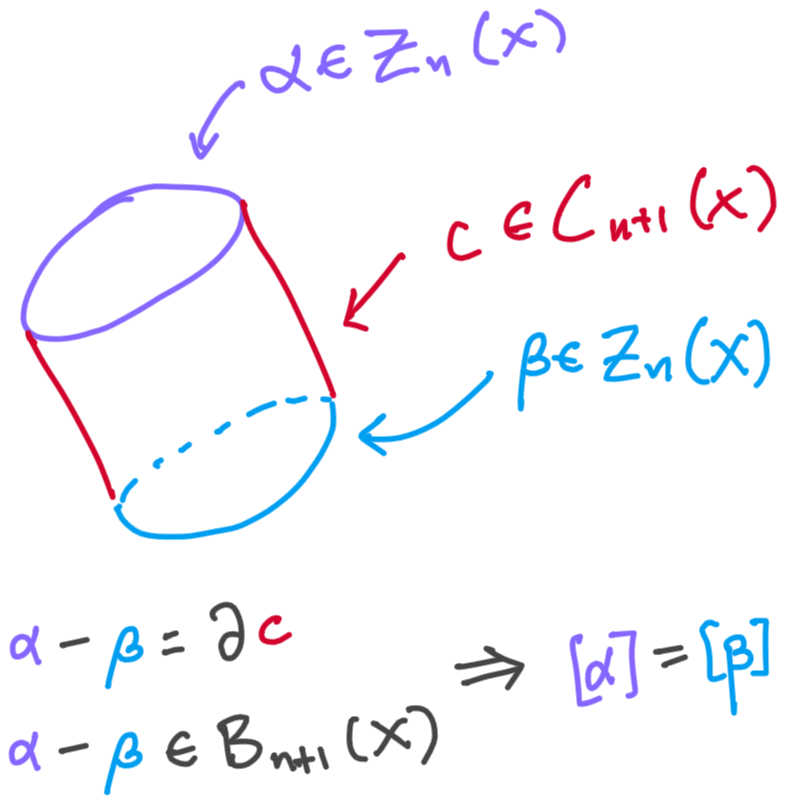
\includegraphics[width=0.4\linewidth]{Homología/H1.png}
	\end{figure}
	\begin{ejer}[Función inducida]
		Si $(C_\bullet{},\partial)\xrightarrow f(C'_\bullet{},\partial')$ es un homeomorfismo, entonces $f(Z_p)\subseteq Z'_p$ y $f(B_p)\subseteq B'_p$ así que la función inducida
		\begin{align*}
			\bar f_p:H_p(C_\bullet{})\to & H_p(C_\bullet{})\\
			a+B_p\mapsto& f_p(a)+B'_p
		\end{align*}
		está bien definida.
		Si además tenemos un segundo homomorfismo $(C'_\bullet,\partial')\xrightarrow{g}(C''_\bullet,\partial'')$, entonces $\overline{g\circ f}=\bar g\circ\bar f$. Y por último, $\overline{Id}_{C_p}=Id_{H_p(C)}$.
	\end{ejer}
	Con este ejercicio comenzamos a ver las propiedades funtoriales de la homología, aunque por ahora no profundizaremos en este lenguaje.
	\section{Sucesiones exactas}
	\begin{defn}
		Decimos que la sucesión 
		\[
		\begin{tikzcd}
			\cdots \arrow{r} & C_p \arrow{r}{f_p} & C_{p-1} \arrow{r}{f_{p-1}} & C_{p-2} \arrow{r} & \cdots
		\end{tikzcd}
		\]
		es \textbf{exacta en $C_p$} si  $\text{img }f_p=\ker{f_{p-1}}$. Y la sucesión es \textbf{exacta} si es exacta en todos los $C_p$. Esto sucede si y sólo si $H_p(C_\bullet{})=0$ para todo $p\in\mathbb{Z}$.
	\end{defn}
	\begin{obs}\leavevmode
		\begin{itemize}
			\item El grupo de homología mide qué tan lejos está la sucesión de ser exacta.
			\item La sucesión puede ser "finita", o sea pueden haber muchos módulos que son cero.
		\end{itemize}
	\end{obs}
	\begin{defn}
		Una sucesión exacta de la forma \[0\to P\to Q\to R\to 0\] se llama \textbf{sucesión exacta corta}. Las sucesiones exactas infinitas en ambas direcciones se llaman \textbf{sucesiones exactas largas}.
	\end{defn}
	\begin{prop}\leavevmode
		\begin{enumerate}
			\item $0\to A\xrightarrow{\alpha}B$ es exacta si y sólo si $\ker{\alpha}=0$, es decir $\alpha $ es inyectiva.
			\item $A\xrightarrow{\alpha}B\to 0$ es exacta si y sólo si $\text{img }{\alpha}=B$, es decir $\alpha $ es suprayectiva.
			\item $0\to A\xrightarrow{\alpha}B\to 0$ es exacta si y sólo si $\alpha $ es un isomorfismo por los dos incisos anteriores.
			\item $0\to A\xrightarrow{\alpha}B\xrightarrow{\beta} C\to0$ es exacta si y sólo si $\alpha$ es inyectiva, $\beta$ es suprayectiva y $\ker\beta=\text{img }\alpha$, de manera que $\beta$ induce un isomorfismo $C\cong B/\text{img }\alpha$.
			
			Si pensamos que $\alpha$ es la inclusión de $A$ como subgrupo de $B$, podemos escribir $C\cong B/A$ .
		\end{enumerate}
	\end{prop}
	\begin{obs}[Primer teorema de isomorfismo] Si $M'\subseteq M$, entonces
		\[
		\begin{tikzcd}
			0 \arrow{r} & M' \arrow[hookrightarrow]{r} & M \arrow[twoheadrightarrow]{r} & M/M' \arrow{r} & 0
		\end{tikzcd}
		\]
		es una sucesión exacta.
	\end{obs}
	\section{Homotopía}
	\begin{defn}
		Dos homomorfismos 
		\begin{align*}
			f,g:(C_\bullet,\partial)\to(C'_\bullet,\partial')
		\end{align*}
		son \textbf{homotópicos} si existen homomorfismos $H_p:C_p\to C'_{p+1}$ para toda $p\in\Z$ tales que \[f_p-g_p=\partial'_{p+1}H_p+H_{p-1}\partial_p\] Estas flechas se pueden visualizar aquí:
		\[\begin{tikzcd}[column sep=large, row sep=large]
			\cdots \arrow{r} & C_{p+1} \arrow{r}{\partial_{p+1}} \arrow{d}[left]{f_{p+1}-g_{p+1}} & C_p \arrow{r}[blue]{\partial_p} \arrow{d}[right,red]{f_p-g_p} \arrow{ld}[left,blue]{H_p} & C_{p-1} \arrow{r} \arrow{d}[right]{f_{p-1}-g_{p-1}} \arrow{ld}[right,blue]{H_{p-1}} & \cdots \\
			\cdots \arrow{r} & C'_{p+1} \arrow{r}[below,blue]{\partial'_{p+1}} & C'_p \arrow{r}[below]{\partial_p'} & C'_{p-1} \arrow{r} & \cdots
		\end{tikzcd}
		\]
		Así que la suma de las flechas azules es igual a la flecha roja. (No estamos diciendo que el diagrama sea conmutativo).
	\end{defn}
	\begin{lema}
		Con la notación de arriba, $\bar f_p=\bar g_p:H_p(C_\bullet)\to H_(C'_\bullet)$. Es decir, funciones homotópicas inducen funciones iguales en homología.
	\end{lema}
	\section{El lema de la serpiente}
	\begin{lema}[de la serpiente]Consideremos el diagrama conmutativo de $R$-módulos y supongamos que sus filas son exactas:
		\[
		\begin{tikzcd}
			&Z_1'\arrow{r}{\phi'}\arrow{d}{\partial_1}&Z_2'\arrow{r}{\psi'}\arrow{d}{\partial_2}&Z_3'\arrow{r}\arrow{d}{\partial_3}&0\\
			0\arrow{r}&Z_1\arrow{r}[below]{\phi}&Z_2\arrow{r}[below]{\psi}&Z_3&
		\end{tikzcd}
		\]
		Entonces existe un homomorfismo $\delta_*:\ker\partial_3\to Z_1/\img\partial_1$ tal que
		\[\begin{tikzcd}
			\ker\partial_1\arrow{r}{\phi''}&\ker\partial_2\arrow{r}{\phi''}&\ker\partial_3\arrow{r}{\delta_*}&Z_1/\img\partial_1\arrow{r}{\bar\phi}&Z_2/\img\partial_2\arrow{r}{\bar\psi}&Z_3/\img\partial_3
		\end{tikzcd}\]
		es exacta, donde $\phi''$ y $\psi''$ son las restricciones de $\phi'$ y $\psi'$, y $\bar\phi$ y $\bar\psi$ son homomorfismos inducidos por $\phi$ y $\psi$. ¿Dónde está la serpiente?
	
		
		\[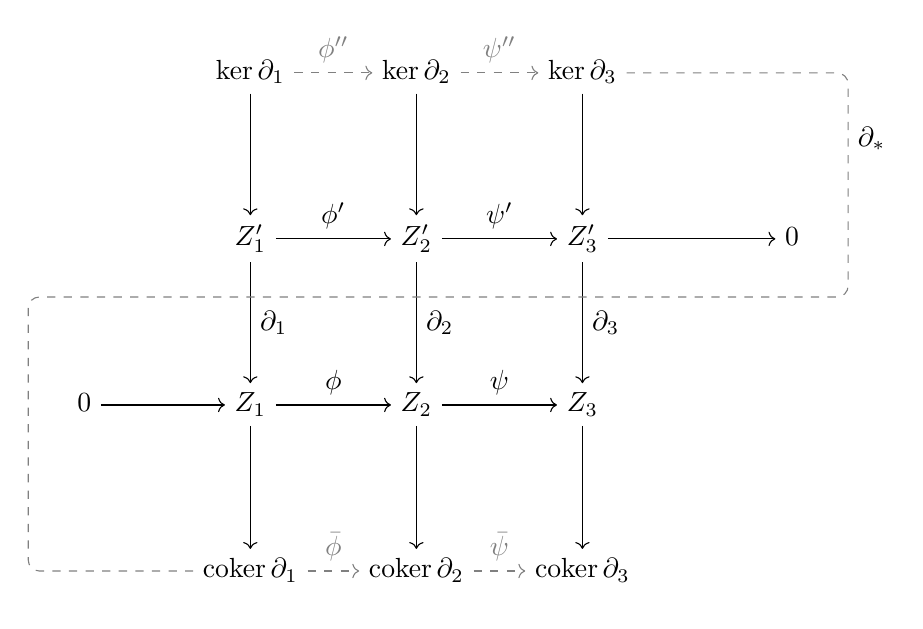
\begin{tikzpicture}
			\matrix[matrix of math nodes,column sep={60pt,between origins},row
			sep={60pt,between origins},nodes={asymmetrical rectangle}] (s)
			{
				&|[name=ka]| \ker \partial_1 &|[name=kb]| \ker \partial_2 &|[name=kc]| \ker \partial_3 \\
				%
				&|[name=A]| Z_1' &|[name=B]| Z_2' &|[name=C]| Z_3' &|[name=01]| 0 \\
				%
				|[name=02]| 0 &|[name=A']| Z_1 &|[name=B']| Z_2 &|[name=C']| Z_3 \\
				%
				&|[name=ca]| \coker \partial_1 &|[name=cb]| \coker \partial_2 &|[name=cc]| \coker \partial_3 \\
			};
			\draw [->]    (ka) edge (A)
			(kb) edge (B)
			(kc) edge (C)
			(A) edge node[auto] {\(\phi'\)} (B)
			(B) edge node[auto] {\(\psi'\)} (C)
			(C) edge (01)
			(A) edge node[auto] {\(\partial_1\)} (A')
			(B) edge node[auto] {\(\partial_2\)} (B')
			(C) edge node[auto] {\(\partial_3\)} (C')
			(02) edge (A')
			(A') edge node[auto] {\(\phi\)} (B')
			(B') edge node[auto] {\(\psi\)} (C')
			(A') edge (ca)
			(B') edge (cb)
			(C') edge (cc)
			;
			\draw[->,gray,dashed] (ka) edge node[auto] {\(\phi''\)}(kb)
			(kb) edge node[auto] {\(\psi''\)}(kc)
			(ca) edge node[auto] {\(\bar\phi\)} (cb)
			(cb) edge node[auto] {\(\bar\psi\)} (cc)
			;
			\draw[gray,dashed,rounded corners] (kc) -| node[auto,text=black,pos=.7]
			{\(\partial_*\)} ($(01.east)+(.5,0)$) |- ($(B)!.35!(B')$) -|
			($(02.west)+(-.5,0)$) |- (ca);
		\end{tikzpicture}\]
		donde $\coker\partial_i=Z_i/\partial_i$. (Este diagrama fue tomado de  \href{https://tex.stackexchange.com/questions/3892/how-do-you-draw-the-snake-arrow-for-the-connecting-homomorphism-in-the-snake-l}{\textbf{internet}}).
	\end{lema}
	\begin{obs}
		Intuitivamente, el $\coker$ nos da información de qué tan lejos está un homomorfismo de ser suprayectivo.
	\end{obs}
%\chapter{El teorema fundamental del álgebra homológica}
\section{Teorema fundamental del álgebra homológica}
	Primero introduciremos algo de notación
	\begin{defn}
		Diremos que una sucesión de complejos de cadena
		\[\begin{tikzcd}
			&\cdots\arrow{r}&C_\bullet\arrow{r}{f}&D_\bullet\arrow{r}{g}&E_\bullet\arrow{r}&\cdots
		\end{tikzcd}\]
		es exacta en $D_\bullet$ si 
		\[\begin{tikzcd}
			&\cdots\arrow{r}&C_p\arrow{r}{f_p}&D_p\arrow{r}{g_p}&E_p\arrow{r}&\cdots
		\end{tikzcd}\]
		es exacta para todo $p\in\Z$
	\end{defn}
	\begin{teo}[fundamental del álgebra homológica]
		Si 
		\[\begin{tikzcd}
			&\cdots\arrow{r}&A_\bullet\arrow{r}{\phi}&B_\bullet\arrow{r}{\psi}&C_\bullet\arrow{r}&\cdots
		\end{tikzcd}\]
		es una sucesión exacta de complejos de cadena, entonces existen homomorfismos \[\partial_{*p}:H_p(C.)\to H_{p-1}(A.)\]
		tales que la sucesión
		\[\begin{tikzcd}
			&\cdots\arrow{r}&H_p(A_\bullet)\arrow{r}{\bar\phi_p}&H_p(B_\bullet)\arrow{r}{\bar\psi_p}&H_p(C_\bullet)\arrow{r}{\delta_{*p}}&H_{p-1}(A_\bullet)\arrow{r}{\bar\phi_{p-1}}&H_{p-1}(B_\bullet)\arrow{r}&\cdots
		\end{tikzcd}\]
		es exacta.
	\end{teo}
	En el siguiente diagrama conmutativo se ve claramente qué está pasando:
	\[
	\begin{tikzcd}
		& & 0 \arrow{d} & 0 \arrow{d} & 0 \arrow{d} & \\
		& \cdots \arrow{r} & A_{p+1} \arrow{r}{\partial_{p+1}} \arrow{d}{i_{p+1}} & A_p \arrow{r}{\partial_p} \arrow{d}{i_p} & A_{p-1} \arrow{r} \arrow{d}{i_{p-1}} & \cdots \\
		& \cdots \arrow{r} & B_{p+1} \arrow{r}{\partial_{p+1}} \arrow{d}{j_{p+1}} & B_p \arrow{r}{\partial_p} \arrow{d}{j_p} & B_{p-1} \arrow{r} \arrow{d}{j_{p-1}} & \cdots \\
		& \cdots \arrow{r} & C_{p+1} \arrow{r}{\partial_{p+1}} \arrow{d} & C_p \arrow{r}{\partial_p} \arrow{d} & C_{p-1} \arrow{r} \arrow{d} & \cdots \\
		& & 0 & 0 & 0 & \\
	\end{tikzcd}
	\]

\section{Natrualidad del homomorfismo de conexión}
	\begin{teo}[Naturalidad del homomorfismo de conexión]
		\[\begin{tikzcd}
			&0\arrow{r}&A_\bullet\arrow{r}{i}\arrow{d}{f}&B_\bullet\arrow{r}{j}\arrow{d}{g}&C_\bullet\arrow{r}\arrow{d}{h}&0\\
			&0\arrow{r}&A'_\bullet\arrow{r}&B'_\bullet\arrow{r}&C'_\bullet\arrow{r}&0
		\end{tikzcd}\]
		donde las filas son exactas.\par
		Entonces, el siguiente diagrama conmuta
		\[\begin{tikzcd}[column sep=small, row sep=large]
			& \cdots \arrow{r} & H_p(A) \arrow{r} \arrow{d}{\bar{f}} & H_p(B) \arrow{r} \arrow{d}{\bar{g}} & H_p(C) \arrow{r}{\delta_*} \arrow{d}{\bar{h}} & H_{p-1}(A) \arrow{r} \arrow{d}{\bar{f}} & H_{p-1}(B) \arrow{r} \arrow{d}{\bar{g}} & H_{p-1}(C) \arrow{r} \arrow{d}{\bar{h}} & \cdots \\
			& \cdots \arrow{r} & H_p(A') \arrow{r} & H_p(B') \arrow{r} & H_p(C') \arrow{r} & H_{p-1}(A') \arrow{r} & H_{p-1}(B') \arrow{r} & H_{p-1}(C') \arrow{r} & \cdots
		\end{tikzcd}\]
	\end{teo}
	Parece que ésta es una propiedad relacionada con la estructura de funtor de la homología.
\section{Lema de los cinco}
	\begin{lema}[de los cinco]
		Consideremos el diagrama conmutativo con filas exactas
		\[\begin{tikzcd}
			M_5\arrow{r}{f_5}\arrow{d}{h_5}&M_4\arrow{r}{f_4}\arrow{d}{h_4}&M_3\arrow{r}{f_3}\arrow{d}{h_3}&M_2\arrow{r}{f_2}\arrow{d}{h_2}&M_1\arrow{d}{h_1}\\
			N_5\arrow{r}{g_5}&N_4\arrow{r}{g_4}&N_3\arrow{r}{g_3}&N_2\arrow{r}{g_2}&N_1
		\end{tikzcd}\]
		Si $h_5,h_4,h_2$ y $h_1$ son isomorfismos, entonces $h_3$ también.
	\end{lema}
	¿En dónde se usará esto?

\chapter{Homología singular}
\section{Simplejos}
	Comenzaremos definiendo varios conceptos nuevos. Fijemos un entero $n\geq0$. Un \textbf{$n$-simplejo} es el convexo más pequeño en $\R^m$ ($m>n$) que contiene $n+1$ puntos $v_0,...,v_n$ que no viven en un hiperplano de dimensión menor que $n$.
	\begin{figure}[H]
		\centering
		\begin{subfigure}{0.23\textwidth}
			\centering
			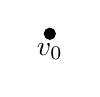
\begin{tikzpicture}[>=latex]
				% TikZ code for the 0-simplex
				\coordinate[label=below:$v_0$] (v0) at (0,0);
				\draw[fill=black] (v0) circle (2pt);
			\end{tikzpicture}
			\caption*{0-simplejo}
		\end{subfigure}
		\begin{subfigure}{0.23\textwidth}
			\centering
			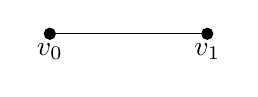
\begin{tikzpicture}[>=latex]
				% TikZ code for the 1-simplex
				\coordinate[label=below:$v_0$] (v0) at (0,0);
				\coordinate[label=below:$v_1$] (v1) at (2,0);
				\foreach \vertex in {v0,v1}
				\draw[fill=black] (\vertex) circle (2pt);
				\draw (v0) -- (v1);
			\end{tikzpicture}
			\caption*{1-simplejo}
		\end{subfigure}
		\begin{subfigure}{0.23\textwidth}
			\centering
			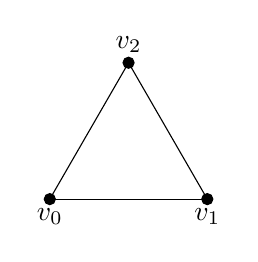
\begin{tikzpicture}[>=latex]
				% TikZ code for the 2-simplex
				\coordinate[label=below:$v_0$] (v0) at (0,0);
				\coordinate[label=below:$v_1$] (v1) at (2,0);
				\coordinate[label=above:$v_2$] (v2) at (1,{sqrt(3)});
				\foreach \vertex in {v0,v1,v2}
				\draw[fill=black] (\vertex) circle (2pt);
				\draw (v0) -- (v1);
				\draw (v1) -- (v2);
				\draw (v0) -- (v2);
			\end{tikzpicture}
			\caption*{2-simplejo}
		\end{subfigure}
		\begin{subfigure}{0.23\textwidth}
			\centering
			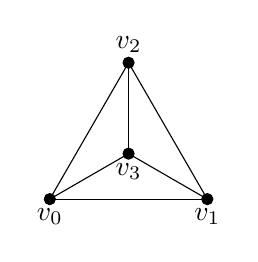
\begin{tikzpicture}[line join=bevel, scale=2]
				\coordinate[label=below:$v_0$] (v0) at (0,0);
				\coordinate[label=below:$v_1$] (v1) at (1,0);
				\coordinate[label=above:$v_2$] (v2) at (0.5,{sqrt(3)/2});
				\coordinate[label=below:$v_3$] (v3) at (0.5,{sqrt(3)/6});
				
				\draw (v1) -- (v2);
				\draw (v2) -- (v3);
				\draw (v0) -- (v1);
				\draw(v0) -- (v2);
				\draw (v0) -- (v3);
				\draw (v1) -- (v3);
				\draw (v2) -- (v3);
				
				% Vertices circles
				\foreach \vertex in {v0,v1,v2,v3}
				\draw[fill=black] (\vertex) circle (1pt);
			\end{tikzpicture}
			\caption*{3-simplejo}
		\end{subfigure}
	\end{figure}
		Lo denotaremos por $[v_0,…,v_n]$ y diremos que 	 $v_0,…,v_n$ son sus \textbf{vértices}. Y podemos escribirlo así: $[v_0,...,v_n]=\{t_0v_0+…+t_nv_n|t_i\geq0,t_0+…+t_n=1\}$.
		
		El \textbf{$n$-simplejo estándar} es $\Delta^n:=[e_1,…,e_n]$ donde $e_1,…,e_n$ es la base canónica de $\R^{n+1}$.
		
	\begin{figure}[H]
		\centering
		\begin{subfigure}{0.3\textwidth}
			\centering
			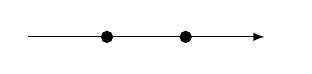
\begin{tikzpicture}[>=latex]
				% Axis
				\draw[->] (-1,0) -- (2,0) node[right]{};
				
				% Vertices
				\coordinate (v0) at (0,0);
				\coordinate (v1) at (1,0);
				
				% Edge
				\draw (v0) -- (v1);
				
				% Vertices circles
				\foreach \vertex in {v0,v1}
				\draw[fill=black] (\vertex) circle (2pt);
			\end{tikzpicture}
			\caption*{1-simplejo estándar}
		\end{subfigure}
		\begin{subfigure}{0.3\textwidth}
			\centering
			\begin{tikzpicture}[>=latex]
				% Axes
				\draw[->] (0,0) -- (2,0) node[right]{$x$};
				\draw[->] (0,0) -- (0,2) node[above]{$y$};
				
				% Vertices
				\coordinate (v0) at (1,0);
				\coordinate (v1) at (0,1);
				
				% Edges
				\draw (v0) -- (v1);
				
				% Vertices circles
				\foreach \vertex in {v0,v1}
				\draw[fill=black] (\vertex) circle (2pt);
			\end{tikzpicture}
			\caption*{2-simplejo estándar}
		\end{subfigure}
		\begin{subfigure}{0.3\textwidth}
			\centering
			\begin{tikzpicture}[>=latex]
				% Axes
				\draw[->] (0,0,0) -- (2,0,0) node[right]{$y$};
				\draw[->] (0,0,0) -- (0,2,0) node[above]{$z$};
				\draw[->] (0,0,0) -- (0,0,2) node[below left]{$x$};
				
				% Vertices
				\coordinate (v0) at (1,0,0);
				\coordinate (v1) at (0,1,0);
				\coordinate (v2) at (0,0,1);
				
				% Edges
				\draw (v0) -- (v1) -- (v2) -- cycle;
				
				% Vertices circles
				\foreach \vertex in {v0,v1,v2}
				\draw[fill=black] (\vertex) circle (2pt);
			\end{tikzpicture}
			\caption*{3-simplejo estándar}
		\end{subfigure}
	\end{figure}
		Y observemos que $\Delta^n=\{(t_0,…,t_n)\in\R^{n+1}|t_0+…+t_n=1\}$
	Para nosotros el orden de los vértices en $[v_0,…,v_n]$ es importante y siempre hay que tenerlo en mente.
	
	Dado un $n$-simplejo siempre tenemos la función:
	\begin{align*}
		(v_0,…,v_n):\Delta^n&\to[v_0,…,v_n]\\
		(t_0+…+t_n)&\mapsto t_0v_0+…+t_nv_n
	\end{align*}
	Y diremos que $(t_0,\cdots+t_n$ son las \textbf{coordenadas baricéntricas} del punto $t_0v_0+…+t_nv_n\in[v_0,…,v_n]$.
	
	Una \textbf{cara} de $[v_0,…,v_n]$ es el subsimplejo de generado por cualquier subconjunto no vacío de ${v_0,…,v_n}$. Cualquier cara 1-dimensional $[v_i,v_j]$ con $i<j$ vamos a considerarla orientada en orden ascendente:
	\vspace*{.7cm}
	
	\begin{center}
	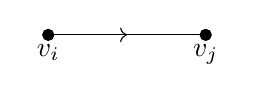
\begin{tikzpicture}
		%Vertices
		\coordinate[label=below:$v_i$] (vi) at (0,0);
		\coordinate[label=below:$v_j$] (vj) at (2,0);
		
		% Vertices circles
		\foreach \vertex in {vi,vj}
		\draw[fill=black] (\vertex) circle (2pt);
	
		% Edge
		\draw[postaction={decorate, decoration={markings, mark=at position 0.5 with {\arrow{>}}}}] (vi) -- (vj);
	\end{tikzpicture}
	\hspace{1cm}
	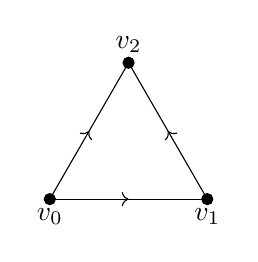
\begin{tikzpicture}
		% Vertices
		\coordinate[label=below:$v_0$] (v0) at (0,0);
		\coordinate[label=below:$v_1$] (v1) at (2,0);
		\coordinate[label=above:$v_2$] (v2) at (1,{sqrt(3)});
		
		% Vertices circles
		\foreach \vertex in {v0,v1,v2}
		\draw[fill=black] (\vertex) circle (2pt);
		
		% Edges
		\draw[postaction={decorate, decoration={markings, mark=at position 0.5 with {\arrow{>}}}}] (v0) -- (v1);
		\draw[postaction={decorate, decoration={markings, mark=at position 0.5 with {\arrow{>}}}}] (v1) -- (v2);
		\draw[postaction={decorate, decoration={markings, mark=at position 0.5 with {\arrow{>}}}}] (v0) -- (v2);
	\end{tikzpicture}
	\hspace{1cm}
	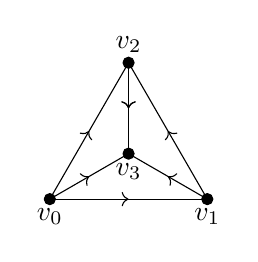
\begin{tikzpicture}[line join=bevel, scale=2]
		\coordinate[label=below:$v_0$] (v0) at (0,0);
		\coordinate[label=below:$v_1$] (v1) at (1,0);
		\coordinate[label=above:$v_2$] (v2) at (0.5,{sqrt(3)/2});
		\coordinate[label=below:$v_3$] (v3) at (0.5,{sqrt(3)/6});
		
	
		\draw[postaction={decorate, decoration={markings, mark=at position 0.5 with {\arrow{>}}}}] (v1) -- (v2);
		\draw[postaction={decorate, decoration={markings, mark=at position 0.5 with {\arrow{>}}}}] (v2) -- (v3);
		\draw[postaction={decorate, decoration={markings, mark=at position 0.5 with {\arrow{>}}}}] (v0) -- (v1);
		\draw[postaction={decorate, decoration={markings, mark=at position 0.5 with {\arrow{>}}}}] (v0) -- (v2);
		\draw[postaction={decorate, decoration={markings, mark=at position 0.5 with {\arrow{>}}}}] (v0) -- (v3);
		\draw[postaction={decorate, decoration={markings, mark=at position 0.5 with {\arrow{>}}}}] (v1) -- (v3);
		\draw[postaction={decorate, decoration={markings, mark=at position 0.5 with {\arrow{>}}}}] (v2) -- (v3);
		
		% Vertices circles
	\foreach \vertex in {v0,v1,v2,v3}
	\draw[fill=black] (\vertex) circle (1pt);
	\end{tikzpicture}
	\end{center}
	
	¿Cómo quedan orientadas las caras de dimensión 2?
	
\section{El complejo de cadenas singulares}
	Tomemos un espacio topológico  $X$  y un anillo asociativo con unidad $R$. Un \textbf{$n$-simplejo singular} es una función $\sigma:\Delta^n\to X$.
	
	El término ``singular" proviene de que no se le imponen condiciones a la función $\sigma$ salvo continuidad. Esto quiere decir que un simplejo singular puede verse bastante diferente de como lo imaginamos inicialmente.
	
	Definamos el siguiente conjunto 
	\[C_n(X):=\left\{\sum_{i=1}^mr_i\sigma_i|m\in\Z,r_i\in\R,\sigma_i\text{ es un simplejo singular}\right\}\]
	Que es el $R$-módulo libre generado por el conjunto de $n$-simplejos singulares. Los elementos de $C_n$ se llaman $n$-cadenas singulares. Queremos construir la siguiente sucesión:
	\begin{equation}\label{eq2.1}\begin{tikzcd}
		\cdots\arrow{r}&C_{n+1}(X)\arrow{r}{\partial_{n+1}}&C_n(X)\arrow{r}{\partial_n}&C_{n-1}(X)\arrow{r}{\partial{n-1}}&\cdots\arrow{r}{\partial_1}&C_0(X)
	\end{tikzcd}\end{equation}
	Para lo cual basta definir
	$\partial_n:C_n(X)\to C_{n-1}(X)$ como sigue: para un $n$-simplejo singular $\sigma:\Delta^n=[v_0,\ldots,v_n]\to X$,
	\[\partial_n(\sigma)=\sum_{i=0}^n(-1)^i\sigma|[v_0,\ldots,\hat{v}_i,\ldots,v_n]\]
	Donde $\sigma|[v_0,\ldots,\hat{v}_i,\ldots,v_n]$ es el siguiente $n-1$-simplejo singular: primero tomemos la $n-1$-cara de $\Delta^n$ que se obtiene al quitar el vértice $v_i$, es decir, $[v_0,\ldots,v_{i-1},v_{i+1},\ldots,v_n]$. Y luego simplemente componemos:
	$\partial_n:C_n(X)\to C_{n-1}(X)$ como sigue: para un $n$-simplejo singular $\partial_n:C_n(X)\to C_{n-1}(X)$ como sigue: para un $n$-simplejo singular $\sigma:\Delta^n=[v_0,\ldots,v_n]\to X$,
	\[\partial_n(\sigma)=\sum_{i=0}^n(-1)^i\sigma|[v_0,\ldots,\hat{v}_i,\ldots,v_n]\]
	Donde $\sigma|[v_0,\ldots,\hat{v}_i,\ldots,v_n]$ es el siguiente $n-1$-simplejo singular: primero tomemos la $n-1$-cara de $\Delta^n$ que se obtiene al quitar el vértice $v_i$, es decir, $[v_0,\ldots,\hat{v}_i,\ldots,v_n]:= [v_0,\ldots,v_{i-1},v_{i+1},\ldots,v_n]$. Y luego simplemente componemos:
	\[
	\begin{tikzcd}
		{[v_0,\ldots,v_n]} \arrow{r}{\sigma} & X \\
		{[v_0,\ldots,\hat{v}_i,\ldots,v_n]}\arrow[u,hook]&{[v_0,\ldots,v_{n-1}]}=\Delta^{n-1}\arrow{l}\arrow{u}[swap]{\sigma|[v_0,\ldots,\hat{v}_i,\ldots,v_n]}
		\arrow[from=1-1, to=2-2, phantom, "\circlearrowright"]
	\end{tikzcd}
	\]
	Donde la flecha de abajo es la función obvia: manda los vértices en orden y se brinca el $i$-ésimo. Y bueno, así queda definida la función $\partial_n$ en la base de $C_n$, y simplemente extendemos por linealidad a todo $C_n$. Ahora veamos una proposición:
	\begin{prop}
		$\partial_{n-1}\circ\partial_n=0$
	\end{prop}
	Con lo que la sucesión \eqref{eq2.1} es un complejo de cadenas que podemos llamar el \textbf{complejo de cadenas singulares de $X$}, que denotaremos por $C_\bullet(X)$. Y ahora podemos considerar sus grupos de homología y definir \[H_n(X;R):=H_n(C_\bullet(X))\] como el \textbf{$n$-ésimo grupo de homología singular de $X$ con coeficientes en $R$.}
\section{Primeras propiedades de la homología}
\subsection{La homología y las componentes arco-conexas}
\begin{prop}
	Sea $X=\bigsqcup X_i$ la descomposición en componentes arco-conexas del espacio topológico $X$, entonces
	\[H_n(\bigsqcup X_i,R)\cong \bigoplus H_n(X_i,R)\]
\end{prop}
\subsection{El 0-ésimo grupo de homología}
\begin{prop}
	Para cualquier espacio $X$, $H_0(X;R)$ es un suma directa de copias de $R$, una por cada componente arcoconexa.
\end{prop}
\subsection{La homología de un punto}
	 \begin{prop}
	 	Si $X$ consiste de un sólo punto, entonces
	 	\[H_n(X;R)=\begin{cases}R\qquad\text{si   } n=0\\
	 	0\qquad\text{si   } n\neq0
		 \end{cases}\]
	\end{prop}
\section{Homología reducida}
	Considera
	\[\quad...\xrightarrow[]{} C_p\xrightarrow[]{\partial_p} C_{p-1}\xrightarrow[]{\partial_{p-1}} C_{p-2}\to...\to C_1\xrightarrow[]{\partial_1}C_0\xrightarrow[]{\partial_0}R\xrightarrow[]{\varepsilon}0\]
	donde $\varepsilon(\sum n_i\sigma_i)=\sum n_i$ es el \textbf{mapeo de aumentación}.
	
	Va a resultar que $\tilde H_n(X;R)=H_n(X;R)$ para toda $n\geq 1$.
	\vspace{1cm}
	
	\textbf{Sobre la homología reducida del espacio que es un sólo punto}

	Sabemos por la proposición de la homología de un punto que si $X=\{x\}$, entonces $H_0(X)=R$, es decir, $\ker{\partial_0}/\text{img }\partial_1=R$. Esto implica que la sucesión corta $0\to \text{img }\partial_1\xrightarrow[]{\partial_1}\ker\partial_0\xrightarrow[]{\partial_0}R\xrightarrow[]{\varepsilon}0$ es exacta.
	
	\textit{¿Cómo deducimos de aquí que $\tilde H_0(X;R)=0$?} Bueno resulta que como el espacio es un punto, $\partial_1=0$, así que de entrada $\text{img }\partial_1=0$. Luego, en realidad tenemos la sucesión exacta corta $0\to\ker\partial_0\xrightarrow[]{\partial_0}R\xrightarrow[]{\varepsilon}0$ que hace a $\partial_0$ un isomorfismo que en particular es inyectivo.
	
	Como $\tilde H_0=\ker\partial_0/\text{img }\partial_1$, entonces $\tilde H_0(X;R)=0$.
	
	\textbf{Y en general} $H_0(X;R)=\tilde H_0(X;R)\oplus R$

\section{Funtorialidad}
\section{Invarianza homotópica}
\begin{teo}
	Si dos funciones $f,g:X\to Y$ son homotópicas, entonces inducen el mismo homomorfismo $f_*=g_*:H_n(X)\to H_n(Y)$.
\end{teo}
\begin{coro}
	Si dos funciones $f,g:X\to Y$ son homotópicas, entonces inducen el mismo homomorfismo $f_*=g_*:H_n(X)\to H_n(Y)$.
\end{coro}
\section{Homología relativa}
Sean $A\subseteq X$ espacios topológicos. Diremos que $(X,A)$ es una buena pareja. Notemos que $(C_\bullet(A))$ es un subcomplejo de $C_\bullet (X)$, así que podemos definir el complejo relativo
\[
C_\bullet(X,A)=C_\bullet(X)/C_\bullet(A)
\]
Y esto simplemente quiere decir que para toda $n$,
\[
C_n(X,A)=C_n(X)/C_n(A)
\]
de forma que las cadenas en $A$ se vuelven triviales.

Es claro que el n-ésimo operador frontera restringido a $C_n(A)$ se mapea a $C_{n-1}(A)$, (pues la frontera de una cadena en $A$ no podría salirse de $A$). Esto quiere decir que el mapeo frontera está bien definido en el cociente. 
\[
...\to C_{n+1}(X,A)\xrightarrow{\partial_{n+1}}C_n(X,A)\xrightarrow{\partial_n}C_{n-1}(X,A)\to...
\]
Esto induce la homología dada por
\[H_n(X,A)=\ker\partial_n/\text{img }\partial_{n-1}\]
\begin{ejer}
	$H_n(X,\{x_0\})=H_n(X)$.
	
	Ahora lo primero que pasa es que tenemos una sucesión exacta corta a la que aplicaremos el teorema fundamental del álgebra homológica:
%	\[
%	0\to C_\bullet(A)\xhookrightarrow{i}C_\bullet(X)\xtwoheadrightarrow{j}C_\bullet(X,A)\to0
%	\]
	Así que obtenemos la \textbf{sucesión exacta larga de la pareja}
	
	\[
	...\to H_n(A)\xrightarrow{i_{*n}}H_n(X)\xrightarrow{j_{*n}}H_n(X,A)\xrightarrow{\partial_n}H_{n-1}(A)\xrightarrow{i_{*n-1}}H_{n-1}(X)\xrightarrow{i_{*p-1}}...
	\]
	Como primera observación notemos que si los grupos de homología de la pareja $C_p(X,A)$ fueran triviales, autimáticamente tedríamos que el mapeo inducido por la inclusión sería un isomorfismo. De hecho, esto es un si y sólo si. Así, los grupos de homología miden qué tan diferentes son los grupos de homología de $A$ y los de $X$.
	
	Finalmente agregamos el comentario de que aunque el mapeo $\partial$ que usamos para completar la sucesión exacta larga de la pareja viene del teorema fundamental del álgebra homológica, y al recordar la demostración del teorema nos damos cuenta de que este mapeo actúa exactamente como el operador frontera original de $X$.
\end{ejer}

\section{Escisión}
Sean $Z\subseteq A\subseteq X$ tales que la cerradura de $Z$ está contenida en el interior de $A$. Entonces
\[(X-Z,A-Z)\hookrightarrow (X,A)\]
induce un isomorfismo
\[H_n(X-Z,A-Z)\to H_n(X,A)\qquad\forall n\]
Equivalentemente, para subespacios $A,B\subseteq X$ cuyos interiores cubren a $X$, la inclusión
\[(B,A\cap B)\hookrightarrow (X,A)\]
induce un isomorfismo
\[H_n(B,A\cap B)\to H_n(X,A)\qquad\forall n\]
\begin{defn} Decimos que $(X,A)$ es un \textbf{buen par} si $A$ es cerrado y es retracto fuerte por deformación de una vecindad en $X$.
\end{defn}

El arete hawaiiano no es un buen par porque cualquier vecindad del punto de pegado contiene un círculo entero, así que no se puede retraer por deformación.

\begin{teo}Sea $(X,A)$ un buen par, entonces
\[q:(X,A)\to(X/A,A/A)\]
induce isomorfismos para toda $n$ de la forma
\[q_{*}:H_n(X,A)\to H_n(X/A,A/A)\cong \tilde{H}_n(X/A)\]
donde la tilde denota la homología reducida.
\end{teo}

En la demostración se usa lema de los 5, invarianza homotópica, etc.

\begin{coro}
	 Sea $(X,A)$ un buen par. Entonces tenemos la siguiente sucesión exacta larga:
	\[…\to\tilde H_n(A)\to\tilde H_n(X)\to \tilde H_n(X/A)\to \tilde H_{n-1}(A)\to\tilde H_{n-1}(X)\to \tilde H_{n-1}(X/A)\to\ldots\]
\end{coro}
\begin{teo}[Homología de la esfera]
\[\tilde H_i(S^n;R)=\begin{cases}R\qquad\text{si   } n=i\\
	0\qquad\text{si   } n\neq i
\end{cases}\]
\end{teo}
\begin{teo}[del punto fijo de Bruwer]
	Sean $n\geq2$ y  $f:D^n\to D^n$, entonces $f$ tiene un punto fijo.
\end{teo}

\section{La sucesión de Mayer-Vietoris}
Sea $X$ un espacio topológico y $A,B\subseteq X$ tales que $X=\text{int } A\cup \text{int } B$. Entonces tenemos la siguiente sucesión larga en homología reducida:
\[…\to\tilde H_{n+1}(X)\to\tilde H_n(A\cap B)\to \tilde H_n(A)\oplus \tilde H_n(B)\to \tilde H_{n}(X)\to\tilde H_{n-1}(A\cap B)\to \tilde H_{n-1}(A)\oplus \tilde H_{n-1}(B)\to…\]

\begin{ejem}
	Veamos el toro $S^1\times S^1$ visto como en el examen, con $A=D^2$ y $B=S^1\vee S^1$, casi todos los grupos de homología se hacen cero (aquí hay que usar que la homología de la cuña es la suma de las homologías de los "cuñandos"), y que la homología de $S^1$ es cero cuando el subíndice es mayor o igual que 2. En fin, para $m>2$, $\tilde H_m(X)=0$.
	
	Ahora para la parte que sí nos toca, *Falta*
\end{ejem}

\chapter{Complejos CW}
\section{Construcción}
	Establezcamos algo de notación
	\begin{itemize}
		\item $D^n=\{x\in\mathbb R^n:|x|\leq1\}$ es el $n$-disco cerrado.
		\item $S^n=\{x\in\mathbb R^n:|x|=1\}$ es la $n$-esfera.
		\item $e^n=\{x\in\mathbb R^n:|x|<1\}$ es la $n$-célula abierta o sólo la $n$-célula.
	\end{itemize}
	De tal forma que
	\begin{itemize}
		\item $\partial D^n=S^{n-1}$
		\item $D^n=e^n\cup S^{n-1}$ como conjuntos (no se usa la topología de la unión disjunta)
		\item Y bueno debe ser cierto que $e^0=\{pt\}$.
	\end{itemize}
	\begin{defn}
		Un espacio $X$ es un complejo $CW$ si se puede construir mediante el siguiente procedimiento:
		\begin{enumerate}
			\item Comenzamos con un espacio discreto $X^0$ que se llama el 0-esqueleto.
			\item El $n$-esqueleto $X^n$ lo obtengo a partir del $n-1$-esqueleto $X^{n-1}$ pegando $n$-células $e^n_\alpha$ vía funciones $\varphi_\alpha:S^{n-1}\to X^{n-1}$. Formalmente tenemos el espacio
			\[X^n=X^{n-1}\bigsqcup_\alpha D_\alpha^n\Big/\sim\qquad\qquad x\sim\varphi_\alpha(x)\quad\text{ si }\quad x\in\partial D^n_\alpha\]
			\textit{Realmente es tomar puntos y unirlos con líneas, y luego tomar líneas y rellenar con discos, etc...}
			\item Realmente es tomar puntos y unir líneas entre ellos, y luego pegar puntos o líneas con discos, etc...
		\end{enumerate}
	\end{defn}
	\begin{defn}
		Si $X=X^n$ para algún $n\in\mathbb N$, decimos que $X$ es de dimensión finita y definimos la dimensión de $X$ como la dimensión de la célula más grande que adjunté. Formalmente, $\dim X=\min \{n:X^n=X\}$.
	\end{defn}
	\begin{ejem}
		\begin{itemize}
			\item Los 0-complejos CW son gráficas.
			\item $S^n$ es un complejo CW.
			\item Los espacios proyectivos:
				\begin{align*}
					\mathbb RP^n&=\mathbb R^{n+1}-\{0\}/x\sim\lambda x,\qquad\lambda\in\mathbb R\\
					&=S^n/x\sim-x\\
					&=D^n/x\sim-x,\qquad x\in\partial D^n=S^{n-1}\\
					&=\mathbb RP^{n-1}\cup e^n\\
					&=\mathbb RP^{n-2}\cup e^{n-1}\cup e^n\\
					&=e^0\cup e^1\cup...\cup e^n
				\end{align*}
				donde las funciones de pegado son justamente las antipodales, que ya conocíamos por ser el cubriente universal.
		\end{itemize}
	\end{ejem}
	\begin{ejer}
		Todo complejo $CW$ es semilocalmente simplemente conexo. Es decir, todo complejo $CW$ tiene cubriente universal.
	\end{ejer}
	\begin{defn}
		La función característica es $\Phi_\alpha$:
		\[\begin{tikzcd}
			&e^n_\alpha \ar[rd] \ar[d, "\text{inclusión}"'] & X^{n-1} \sqcup D_\alpha^n \ar[d, "\text{proyección al cociente}"] \\
			&D^n_\alpha \ar[ur] \ar[r, "\Phi_\alpha"'] & X^n
		\end{tikzcd}\]
	\end{defn}
	\begin{defn}
		Sea $X$ un complejo $CW$. Un subcomplejo $Z$ es un subespacio cerrado que además es unión de células de $X$.	
	\end{defn}
	\begin{obs}
		Para un subcomplejo $Z$,
		\begin{itemize}
			\item $Z\subseteq X$ es una buena pareja ($Z$ es retracto por deformación de una vecindad de $X$)
			\item $X/Z$ es un complejo $CW$.
		\end{itemize}
	\end{obs}
	\begin{obs}[Muy importante] $X$ complejo $CW$. El cociente por el $n-1$ esqueleto es una cuña de esferas, tantas como células en el $n-1$ esqueleto. En símbolos, $X^n/X^{n-1}=\bigvee_{\alpha\in I_n}S^n$, donde $I_n$ es el conjunto que indexa las $n-1$-celdas.
	\end{obs}

\section{Homología de complejos CW}
\begin{lema}\leavevmode
	
	\begin{itemize}
		\item \[H_k(X^n,X^{n-1})=\begin{cases}0\qquad\quad\qquad\text{si }k\neq0\\
			\bigoplus_{\alpha\in I_n}R\qquad \text{si } k=n
		\end{cases}\]
		\begin{proof}[Express]
			$H_k=\tilde H_k(X^n/X^{n-1})=\tilde H_k(\bigvee_{\alpha \in I_n}S^n)=\bigoplus_{\alpha\in I_n}H_k(S^n)$
		\end{proof}
		\item $H_k(X^n)=0$ para toda $k>n$. 
		
		Nuevamente, la homología, lo que aclance a ver la homología, lo ve solamente hasta la dimensión del espacio
		\item La inclusión $X^n\hookrightarrow X$ induce un isomorfismo $H_k(X^n)\hookrightarrow H_k(X)\qquad k>n$.
		
		Aquí la idea es que adjuntar células de dimensión mayor que la homología que estamos calculando no cambia la homología. Es decir, para $n>k$ se tiene que $H_k(X\cup D^n)=H_k(X)$.
	\end{itemize}
	\end{lema}
	\begin{proof}
		content...Fijémonos en $(X^n,X^{n-1})$, hay una sucesión exacta corta de la pareja:
		
		\[H_{k+1}(X^n,X^{n-1})\to H_k(X^{n-1})\to H_k(X^n)\to H_k(X^n,X^{n-1})\]
		
		Usando el inciso 1, si $k\neq n,n-1$ entonces $H_k(X^{n-1})\cong H_k(X^n)$.
		
		Bueno para demostrar (2), justamente tenemos $k>n$ y entonces resultará, fijando $k$ y bajando uno por uno, $H_k(X^n)\cong H_k(X^0)$ que es un espacio discreto y la homología de grado mayor que cero en espacios discretos es cero. Terminamos el inciso (2).
		
		Para (3), si $k<n<n+1<n+2<...$, simplemente tenemos que
		\[H_k(X^n)\cong H_k(X^{n+1})\cong...\cong H_k(X^{n+m})\]
		y si pedimos que $X$ sea de dimensión finita entonces terminaremos en algún punto y listo. El caso de dimensión infinita queda para el futuro.
	\end{proof}
	\begin{defn}[Homología celular] Consideremos
		\[\begin{tikzcd}[column sep=tiny]
			& H_{n-1}(X^{n-1}) \arrow[rd, "j_{n-1}"] \\
			H_n(X^n, X^{n-1}) \arrow[ru, "\partial_n"] \arrow[rr, "d_n"] && H_{n-1}(X^{n-1}, X^{n-2}) \arrow[rd, "\partial_{n-1}"] \arrow[rr, "d_{n-1}"] && H_{n-2}(X^{n-2}, X^{n-3}) \\
			& && H_{n-2}(X^{n-2}) \arrow[ru, "j_{n-2}"]
		\end{tikzcd}\]
		Resultará que las flechas horizontales que definimos con los triangulitos, es decir las $d_i$, satisfacen que \[d_{n+1}\circ d_n=0\] así que podemos bautizar el complejo de cadenas $C_\bullet^{CW}(X,R)$. Y ahora podemos definir la homología celular: \[H^{CW}_n(X;R)=H_n(C_\bullet^{CW}(X))\]
	\end{defn}
	\begin{teo}
		\[H_n^{CW}(X;R)\cong H_n(X;R)\qquad\forall n\geq0\]
	\end{teo}
	El primero depende de la estructura celular del espacio $X$, pero el segundo no. Así, la homología de un complejo $CW$ es independiente de la estructura celular.
	\begin{obs}
		content...Estos grupos $H_n(X^n,X^{n-1})$ son las sumas directas de $R$, uno por cada n-celula de $X$ ie $\bigoplus_{n-\text{células de }X}R=\{\sum r_\alpha e^n_\alpha|e^n_\alpha \text{ es una }n\text{-célula }r_\alpha\in R\}$.
	\end{obs}
\end{document}